\documentclass[a4paper,12pt]{article}

%%% Работа с русским языком
\usepackage{cmap}					% поиск в PDF
\usepackage{mathtext} 				% русские буквы в формулах
\usepackage[T2A]{fontenc}			% кодировка
\usepackage[utf8]{inputenc}			% кодировка исходного текста
\usepackage[english,russian]{babel}	% локализация и переносы

%%% Дополнительная работа с математикой
\usepackage{amsfonts,amssymb,amsthm,mathtools} % AMS
\usepackage{amsmath}
\usepackage{icomma} % "Умная" запятая: $0,2$ --- число, $0, 2$ --- перечисление

\usepackage[left = 2cm, right = 2cm, top = 2cm, bottom = 2cm]{geometry}

\usepackage{booktabs}
\usepackage{dcolumn}

%% Номера формул
%\mathtoolsset{showonlyrefs=true} % Показывать номера только у тех формул, на которые есть \eqref{} в тексте.

%% Шрифты
\usepackage{euscript}	 % Шрифт Евклид
\usepackage{mathrsfs} % Красивый матшрифт

%% Свои команды
\DeclareMathOperator{\sgn}{\mathop{sgn}}

%% Перенос знаков в формулах (по Львовскому)
\newcommand*{\hm}[1]{#1\nobreak\discretionary{}
	{\hbox{$\mathsurround=0pt #1$}}{}}

%%% Работа с картинками
\usepackage{graphicx}  % Для вставки рисунков
\graphicspath{{images/}{images2/}}  % папки с картинками
\setlength\fboxsep{3pt} % Отступ рамки \fbox{} от рисунка
\setlength\fboxrule{1pt} % Толщина линий рамки \fbox{}
\usepackage{wrapfig} % Обтекание рисунков и таблиц текстом

%%% Работа с таблицами
\usepackage{array,tabularx,tabulary,booktabs} % Дополнительная работа с таблицами
\usepackage{longtable}  % Длинные таблицы
\usepackage{multirow} % Слияние строк в таблице
\usepackage{upgreek}
\usepackage{enumerate}
\usepackage{ dsfont }

%%% Цветной текст

\usepackage[usenames]{color}
\usepackage{colortbl}
\usepackage[table,xcdraw]{xcolor}

%%% Солнышко

\usepackage[weather]{ifsym}

%%% Гиперссылки

\usepackage{xcolor}
\usepackage{hyperref}
\definecolor{linkcolor}{HTML}{199B03} % цвет ссылок
\definecolor{urlcolor}{HTML}{199B03} % цвет гиперссылок

\hypersetup{pdfstartview=FitH,  linkcolor=linkcolor,urlcolor=urlcolor, colorlinks=true}

\usepackage{minted}

%% Tikz

\usepackage{pgf,tikz,pgfplots}
\pgfplotsset{compat=1.15}
\usepackage{mathrsfs}
\usetikzlibrary{arrows}
\pagestyle{empty}

%%Вставка картинок
\usepackage{graphicx}
\graphicspath{{}}
\DeclareGraphicsExtensions{.pdf,.png,.jpg}


%% эконометрические сокращения
\def \hb{\hat{\beta}}
\DeclareMathOperator{\sVar}{sVar}
\DeclareMathOperator{\sCov}{sCov}
\DeclareMathOperator{\sCorr}{sCorr}


\def \hs{\hat{s}}
\def \hy{\hat{y}}
\def \hY{\hat{Y}}
\def \he{\hat{\varepsilon}}
\def \v1{\vec{1}}
\def \cN{\mathcal{N}}
\def \e{\varepsilon}
\def \z{z}
\def \hb{\hat{\beta}}

\def \hVar{\widehat{\Var}}
\def \hCorr{\widehat{\Corr}}
\def \hCov{\widehat{\Cov}}

\DeclareMathOperator{\tr}{tr}
\DeclareMathOperator*{\plim}{plim}


%% лаг
\renewcommand{\L}{\mathrm{L}}


\usepackage{pgf}
\usepackage{tikz}
\usetikzlibrary{arrows,automata}


% DEFS
\def \mbf{\mathbf}
\def \msf{\mathsf}
\def \mbb{\mathbb}
\def \tbf{\textbf}
\def \tsf{\textsf}
\def \ttt{\texttt}
\def \tbb{\textbb}

\def \wh{\widehat}
\def \wt{\widetilde}
\def \ni{\noindent}
\def \ol{\overline}
\def \cd{\cdot}
\def \bl{\bigl}
\def \br{\bigr}
\def \Bl{\Bigl}
\def \Br{\Bigr}
\def \fr{\frac}
\def \bs{\backslash}
\def \lims{\limits}
\def \arg{{\operatorname{arg}}}
\def \dist{{\operatorname{dist}}}
\def \VC{{\operatorname{VCdim}}}
\def \card{{\operatorname{card}}}
\def \sgn{{\operatorname{sign}\,}}
\def \sign{{\operatorname{sign}\,}}
\def \xfs{(x_1,\ldots,x_{n-1})}
\def \Tr{{\operatorname{\mbf{Tr}}}}
\DeclareMathOperator*{\argmin}{arg\,min}
\DeclareMathOperator*{\argmax}{arg\,max}
\DeclareMathOperator*{\amn}{arg\,min}
\DeclareMathOperator*{\amx}{arg\,max}
\def \cov{{\operatorname{Cov}}}
\DeclareMathOperator{\Var}{Var}
\DeclareMathOperator{\Cov}{Cov}
\DeclareMathOperator{\Corr}{Corr}

\def \xfs{(x_1,\ldots,x_{n-1})}
\def \ti{\tilde}
\def \wti{\widetilde}


\def \mL{\mathcal{L}}
\def \mW{\mathcal{W}}
\def \mH{\mathcal{H}}
\def \mC{\mathcal{C}}
\def \mE{\mathcal{E}}
\def \mN{\mathcal{N}}
\def \mA{\mathcal{A}}
\def \mB{\mathcal{B}}
\def \mU{\mathcal{U}}
\def \mV{\mathcal{V}}
\def \mF{\mathcal{F}}

\def \R{\mbb R}
\def \N{\mbb N}
\def \Z{\mbb Z}
\def \P{\mbb{P}}
%\def \p{\mbb{P}}
\def \E{\mbb{E}}
\def \F{\mbb{F}}
\def \D{\msf{D}}
\def \I{\mbf{I}}
\def \L{\mathcal{L}}

\def \a{\alpha}
\def \b{\beta}
\def \t{\tau}
\def \dt{\delta}
\def \e{\varepsilon}
\def \ga{\gamma}
\def \kp{\varkappa}
\def \la{\lambda}
\def \sg{\sigma}
\def \sgm{\sigma}
\def \tt{\theta}
\def \ve{\varepsilon}
\def \Dt{\Delta}
\def \La{\Lambda}
\def \Sgm{\Sigma}
\def \Sg{\Sigma}
\def \Tt{\Theta}
\def \Om{\Omega}
\def \om{\omega}

\usepackage{graphicx}
\usepackage[referable]{threeparttablex}

%%% Заголовок
\author{Зехов Матвей}
\title{Заметки по многошаговому прогнозированию}
\date{\today}

\begin{document}
	\newpage
\thispagestyle{empty}
\begin{center}
	\textbf{ПРАВИТЕЛЬСТВО РОССИЙСКОЙ ФЕДЕРАЦИИ}\\
	\vspace{2ex}
	\textbf{Федеральное государственное автономное\\ образовательное учреждение высшего образования}
	
	\vspace{2ex}
	
	\textbf{Национальный исследовательский университет \\ <<Высшая школа экономики>>}
	
	\vspace{8ex}
	\begin{flushright}
		Факультет экономических наук\\
		Образовательная программа <<Экономика>>
	\end{flushright}
\end{center}
\vspace{9ex}

\begin{center}
	{\textbf{ДОМАШНЕЕ ЗАДАНИЕ 1
	}}
	\vspace{1ex}
	
	<<Прикладная микроэконометрика>>
\end{center}
\vspace{1ex}
\begin{flushright}
	\noindent
	Студент группы БЭК165\\Зехов Матвей Сергеевич\\
	\vspace{13ex}
	Преподаватель:\\
	Потанин Богдан Станиславович
	
\end{flushright}	

\vfill

\begin{center}
	Москва 2019
	
\end{center}

\newpage
	\tableofcontents
	
\newpage
\section{Часть 1. Теория и гипотезы.}
\begin{enumerate}[\Sun]
	\item Выберите независимые переменные. Теоретически обоснуйте выбор каждой из
	них. Укажите предполагаемые направления эффектов. При этом вам понадобится как
	минимум одна непрерывная переменная и одна дамми переменная (не рекомендуется
	брать больше трех различных переменных, не считая их нелинейных преобразований:
	квадрат, логарифм, перемножение с целью получения переменной взаимодействия и т.д.).
	Приведите по крайней мере две ссылки на научные работы (желательно из Q1
	журналов), изучавшие влияние различных факторов на вероятность брака. Кратко
	опишите методологию и основные результаты этих исследований, а также как ваш выбор
	переменных и сформулированные гипотезы соотносятся с данными результатами. 
	
	Постарайтесь подбирать независимые переменные таким образом, чтобы избежать
	проблемы обратной причинности. То есть ваши независимые переменные должны, в
	теоретическом смысле, влиять на зависимую, а не наоборот. Например, уместно
	предположить, что возраст влияет на вероятность брака. В то же время, скорее всего, не
	количество детей влияет на вероятность брака, а, вполне возможно, наоборот. Поэтому
	возраст можно включить в число независимых переменных, а число детей — не
	желательно
	
	\item Сформулируйте по крайней мере одну гипотезу о наличии эффекта
	взаимодействия и нелинейного эффекта (например, квадратичного). Теоретически
	обоснуйте выдвигаемые вами гипотезы. Включите соответствующие переменные в вашу
	модель.
	
	
	\item Определитесь с тем, будете ли вы предсказывать вероятность брака для
	мужчин и женщин в рамках единой модели, либо остановитесь лишь на одном из полов.
	Обоснуйте свой выбор теоретически.
	
	
	
\end{enumerate}

В этой работе будет рассматриваться вероятность вступления в брак для совершеннолетних мужчин. Для этого были выбраны следующие переменные: возраст в качестве непрерывной переменной и наличие работы в качестве дамми-переменной, а также возраст в квадрате и произведение двух базовых переменных. Модель для мужчин будет оцениваться отдельно от женщин, потому что поведение мужчин и женщин не только отличается возрастом заключения первого брака (Goodwin, P., McGill, B., \& Chandra, A. (2009). Who marries and when?; age at first marriage in the United States, 2002.), но и направление эффектов может различаться по знаку, так как мужчины и женщины воспринимают брак по-разному. 

С возрастом вероятность быть в браке для мужчин повышается, о чём говорят многие исследования. Для проверки гипотезы о наличии нелинейной зависимости от возраста была введена переменная квадрата возраста. Можно предположить, что вероятность вступления в брак максимальна для мужчин среднего возраста, о чём бы говорил значимость этого коэффициента. Трудоустройство мужчины считается одним из самых сильных показателей при прогнозировании вероятность его семейного статуса: работающие мужчины с большей вероятностью будут женаты. Стоит отметить, что в качестве предиктора стоит использовать именно факт наличия работы, а не величину дохода, потому что существует неоднозначный эффект супружеской премии. Направление зависимости до конца не изучено. Существуют исследования, согласно которым факт замужества может влиять на величину труда (Аистов, А. В., \& Коваленко, Н. В. Супружеская премия//XIV Апрельская международная научная конференция по проблемам развития экономики и общества: в 4 кн./отв. ред. ЕГ Ясин, 661-671.), так и наоборот (Chun, H., \& Lee, I. (2001). Why do married men earn more: Productivity or marriage selection?. Economic Inquiry, 39(2), 307-319.). Переменная произведения трудоустройства и возраста позволит изучить совместное влияние двух этих факторов на вероятность вступления в брак. Можно предположить, что для более молодых мужчин наличие работы будет фактором, снижающим вероятность нахождения в браке из-за того, что они либо не ходят в университет, либо совмещают работу и учёбу, а потому у них остаётся меньше времени для формирования семьи. Для более старших мужчин, напротив, наличие работы будет важным показателем, так как это позволит им обеспечивать семью и, возможно, сделает их более привлекательными для заключения брака. 

В статье «Sex Differences in the Entry into Marriage» (Goldscheider, F. K., \& Waite, L. J. (1986). Sex differences in the entry into marriage. American journal of sociology, 92(1), 91-109.) авторы оценивали логистическую модель на выборке 18-29 лет для мужчин, которую они разбили на несколько кластеров для предсказания вероятности «ранней» и «поздней» женитьбы. В качестве объясняющих переменных авторы выбрали расу, образование, трудоустройство, военную службу, образование родителей. В результате они обнаружили, что влияние трудоустройства на вероятность заключения брака положительно для всех возрастов, но сильнее для более старших индивидов. В другой статье «Employment and marriage among inner-city fathers» (Testa, M., Astone, N. M., Krogh, M., \& Neckerman, K. M. (1989). Employment and marriage among inner-city fathers. The Annals of the American Academy of Political and Social Science, 501(1), 79-91.) авторы анализировали, будет ли мужчина жениться на женщине после зачатия с ней первого ребёнка. Для этого авторы строят логистическую регрессию для предсказания вероятности заключения брака в период между зачатием и рождением ребёнка на основе расы, трудоустройства и образования мужчины и других параметров. В результате было замечено, что у трудоустроенного отца в два раза выше вероятность легитимизировать брак до рождения ребёнка.

\section{Часть 2. Обработка данных}
\subsection{}
\Sun  Приведите ваши данные в порядок, удалив пропуски и очистив используемые
переменные от неточностей (осуществляется в коде, в работе это описывать не
обязательно).

\subsection{}
\Sun Рассмотрите доли холостых людей и состоящих в браке. Укажите в таблице
описательные статистики для ваших независимых переменных: отдельно для холостых и
состоящих в браке. Сделайте выводы о различии в распределении независимых
переменных среди индивидов в зависимости от семейного статуса


Ответ. Доля состоящих в браке людей составляет 61\% от выборки.  В таблицах \ref{tab1} и \ref{tab2} приведены описательные статистики для женатых и холостых мужчин. 
\begin{table}[ht]
	\centering
	\resizebox{\textwidth}{!}{%
	\begin{tabular}{|lllllllll|}
		\hline
		age &      work &      alc &      male &    marriage &    workxage &   educ\_high &    educ\_mid &   educ\_other \\ 
		\hline
		Min.   :18.00   & Min.   :0.0000   & Min.   :0.0000   & Min.   :1   & Min.   :1   & Min.   : 0.00   & Min.   :0.0000   & Min.   :0.0000   & Min.   :0.0000   \\ 
		1st Qu.:38.00   & 1st Qu.:0.0000   & 1st Qu.:1.0000   & 1st Qu.:1   & 1st Qu.:1   & 1st Qu.: 0.00   & 1st Qu.:0.0000   & 1st Qu.:0.0000   & 1st Qu.:0.0000   \\ 
		Median :51.00   & Median :1.0000   & Median :1.0000   & Median :1   & Median :1   & Median :34.00   & Median :0.0000   & Median :0.0000   & Median :0.0000   \\ 
		Mean   :50.64   & Mean   :0.6439   & Mean   :0.7522   & Mean   :1   & Mean   :1   & Mean   :28.29   & Mean   :0.2716   & Mean   :0.3791   & Mean   :0.3493   \\ 
		3rd Qu.:62.00   & 3rd Qu.:1.0000   & 3rd Qu.:1.0000   & 3rd Qu.:1   & 3rd Qu.:1   & 3rd Qu.:47.00   & 3rd Qu.:1.0000   & 3rd Qu.:1.0000   & 3rd Qu.:1.0000   \\ 
		Max.   :89.00   & Max.   :1.0000   & Max.   :1.0000   & Max.   :1   & Max.   :1   & Max.   :77.00   & Max.   :1.0000   & Max.   :1.0000   & Max.   :1.0000   \\ 
		\hline
	\end{tabular}%
	
}
\caption{Описательные статистики для женатых \label{tab1} }
\vspace{2em}
	\centering
	\resizebox{\textwidth}{!}{%
	\begin{tabular}{|lllllllll|}
		\hline
		age &      work &      alc &      male &    marriage &    workxage &   educ\_high &    educ\_mid &   educ\_other \\ 
		\hline
		Min.   :18.00   & Min.   :0.0000   & Min.   :0.0000   & Min.   :1   & Min.   :0   & Min.   : 0.00   & Min.   :0.0000   & Min.   :0.0000   & Min.   :0.0000   \\ 
		1st Qu.:25.00   & 1st Qu.:0.0000   & 1st Qu.:0.0000   & 1st Qu.:1   & 1st Qu.:0   & 1st Qu.: 0.00   & 1st Qu.:0.0000   & 1st Qu.:0.0000   & 1st Qu.:0.0000   \\ 
		Median :33.00   & Median :1.0000   & Median :1.0000   & Median :1   & Median :0   & Median :22.00   & Median :0.0000   & Median :0.0000   & Median :0.0000   \\ 
		Mean   :39.12   & Mean   :0.5487   & Mean   :0.6881   & Mean   :1   & Mean   :0   & Mean   :19.47   & Mean   :0.1762   & Mean   :0.3663   & Mean   :0.4575   \\ 
		3rd Qu.:51.00   & 3rd Qu.:1.0000   & 3rd Qu.:1.0000   & 3rd Qu.:1   & 3rd Qu.:0   & 3rd Qu.:33.00   & 3rd Qu.:0.0000   & 3rd Qu.:1.0000   & 3rd Qu.:1.0000   \\ 
		Max.   :92.00   & Max.   :1.0000   & Max.   :1.0000   & Max.   :1   & Max.   :0   & Max.   :77.00   & Max.   :1.0000   & Max.   :1.0000   & Max.   :1.0000   \\ 
		\hline
	\end{tabular}%
}
\caption{Описательные статистики для холостых \label{tab2}}
\end{table}

На основе приведённых статистик можно сделать следующие выводы:

\begin{enumerate}[\Sun]
	\item Средний и медианный возраст женатых мужчин выше, чем неженатых. В общем, ожидаемый результат. Он согласуется с озвученным выше предположением о том, что для мужчин с возрастом растёт вероятность вступления в брак. 
	
	\item Доля занятых среди женатых выше, чем среди неженатых. Скорее всего это связано с необходимостью для мужчины обеспечивать семью и поддерживать достаточный уровень жизни. Женатым сложнее оставить на некоторое время работу, даже при наличии возможности, так как от них зависят и члены семьи.
	
	\item Доля людей, употребляющих алкоголь, выше среди женатых, хотя это не слишком сильно выражено. Возможно, эта разница может быть связана с семейными проблемами
	
	\item Среди женатых выше доля людей с высшим образованием. Это может быть объяснено тем, что наличие ступени обучения повышает вероятность брака в принципе.
\end{enumerate}

\subsection{}
\Sun  Найдите характеристики среднего и медианного индивидов. Результат
представьте в форме таблицы и опишите его словами. Сделайте выводы о различии в
характеристиках между средним и медианным индивидами.


Ответ. В Таблице \ref{tab3} представлены характеристики среднего и медианного индивидов. Как можно видеть, если округлить средние значения бинарных переменных, средний и медианный индивид почти не различаются. Возраст среднего индивида чуть выше, чем у медианного. У обоих есть работа и оба употребляют алкоголь. Также оба женаты.
\begin{table}[ht]
	\centering
		\resizebox{\textwidth}{!}{%
	\begin{tabular}{|rrrrrrrrrr|}
		\hline
		& age & work & alc & male & marriage & workxage & educ\_high & educ\_mid & educ\_other \\ 
		\hline
		Mean & 46.17 & 1 & 1 & 1& 1 & 24.86 & 0 & 0 & 0 \\ 
		Median & 45.00 & 1 & 1 & 1 & 1 & 28.00 & 0 & 0 & 0 \\ 
		\hline
	\end{tabular}
}
\caption{Характеристики среднего и медианного индивидов \label{tab3}}
\end{table}


\subsection{}

\Sun  Отобразите при помощи двух гистограмм различия в распределении одной из
ваших независимых переменных в зависимости от семейного статуса индивида. Сделайте
выводы о различиях в распределении, а также приведите возможное теоретическое
обоснование данных различий. 


Ответ. Для визуализации рассмотрим гистограммы возраста в зависимости от семейного положения индивида. Их можно увидеть на Рис. 1. Как легко заметить, среднее распределения неженатых мужчин действительно смещено влево, но имеет при этом тяжёлый хвост. Это говорит о том, что неженатыми в основном является молодёжь. В целом, это логичный результат, что молодёжь не слишком торопится вступать в брак. Тем не менее, тяжёлый хвост говорит о том, что довольно большой процент мужчин вообще не может в ступить в брак по каким-либо причинам, либо разведены.

Гистограмма распределения женатых мужчин говорит о том, что распределение довольно симметрично. Не слишком много мужчин рано вступает в брак и, очевидно, не слишком много доживает до преклонных лет. Хвосты распределения тоже тяжёлые, но не так сильно, как для неженатых.
\begin{figure}[!h]
	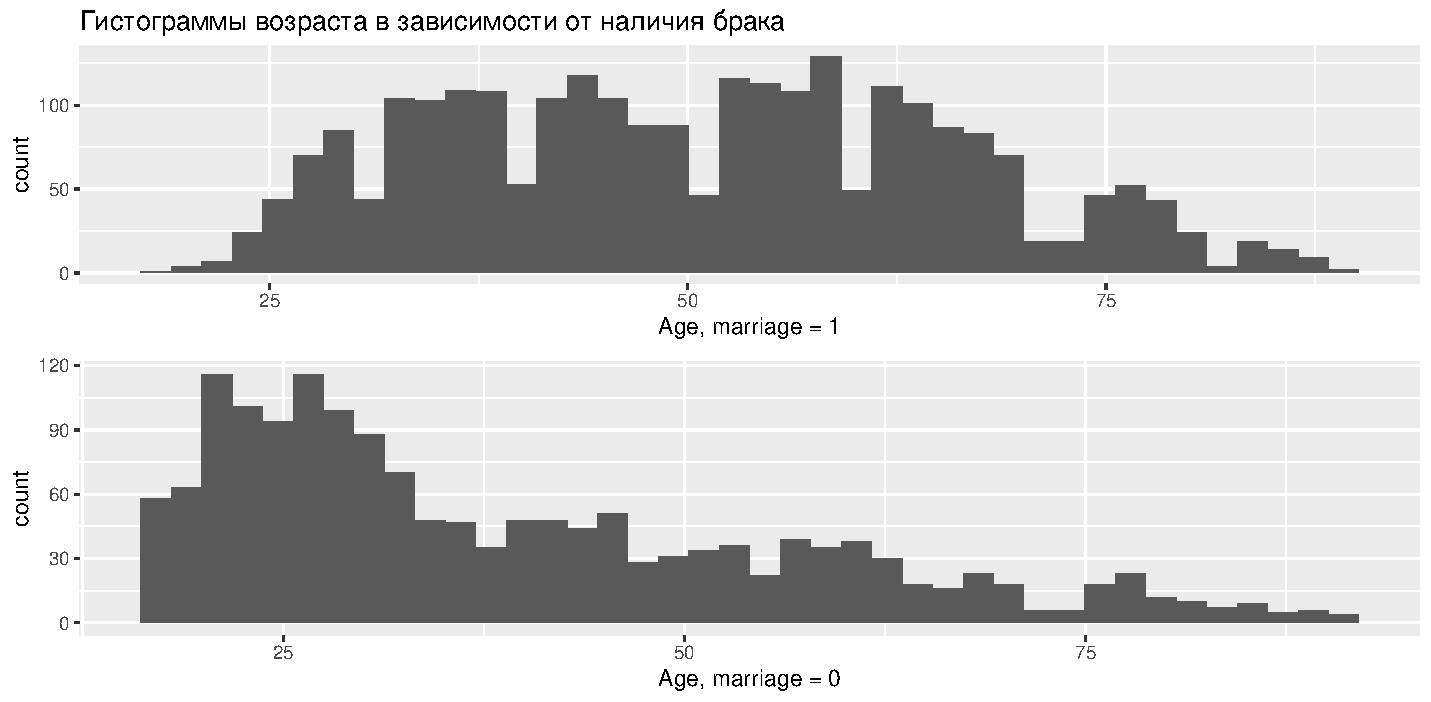
\includegraphics[width=\linewidth]{Histograms}
	\caption{Гистограммы \label{his}}
\end{figure}

\section{}


\subsection{}

\Sun Оцените линейно-вероятностную модель, предварительно записав
регрессионное уравнение. Результат представьте в форме таблицы (можно, например,
использовать выдачу из stata, R или python).


Ответ. Регрессионное уравнение линейно-вероятностной модели:

\[ marriage_i = \beta_0 + \beta_1 age_i + \beta_2 age_i^2 + \beta_3 work_i + \beta_4 workxage_i + \e_i \]

В Таблице 4 представлены результаты оценки этой модели.
\begin{table}[ht]
	\centering
	\begin{tabular}{|rrrrr|rr|}
		\hline
		& Estimate & Std. Error & t value & Pr($>$$|$t$|$) & Metrics & Value \\ 
		\hline
		(Intercept) & -0.9034 & 0.0609 & -14.83 & 0.0000 &R$^2$       & 0.21   \\ 
		age & 0.0514 & 0.0026 & 19.86 & 0.0000 & Adj. R$^2$  & 0.21    \\ 
		I(age\verb|^|2) & -0.0004 & 0.0000 & -15.68 & 0.0000 & Num. obs.   & 4122     \\ 
		work & 0.3648 & 0.0442 & 8.26 & 0.0000 & 	RMSE        & 0.43   \\ 
		workxage & -0.0047 & 0.0010 & -4.90 & 0.0000 &	F-statistic(pval)  &274.2(0.0000) \\
		\hline

	\end{tabular}
\caption{Результаты оценки линейно-вероятностной модели}
\end{table}

\subsection{}

\Sun Скорректируйте оценку ковариационной матрицы оценок регрессионных
коэффициентов при помощи бутстрапа. Объясните причины, по которым необходимо
осуществлять данную корректировку и к каким негативным последствиям может привести
её отсутствие. Результат представьте в форме таблицы (можно, например, использовать
выдачу из stata, R, python).

Ответ. Так как предположение о нормальности ошибок может не соблюдаться, то метод максимального правдободобия может давать несостоятельные и смещённые оценки коэффициентов и ковариационной матрицы, так как правдоподобие будет записано ошибочно. Бутстрап помогает преодолеть эту проблему и получить состоятельные оценки без предположения о нормальности ошибок. Результаты можно видеть в Таблице 5.

\begin{table}[ht]
	\centering
	\begin{tabular}{|rrr|}
		\hline
		& Бутстрапированные s.e. & Старые s.e. \\ 
		  \hline
		(Intercept) & 0.0430 & 0.0609 \\ 
		age & 0.0022 & 0.0026 \\ 
		I(age\verb|^|2) & 0.0000 & 0.0000 \\ 
		work & 0.0370 & 0.0442 \\ 
		workxage & 0.0008 & 0.0010 \\ 
		\hline
	\end{tabular}
\caption{Бутстрапированные и старые стандартные ошибки}
\end{table}

\subsection{}
\Sun Протестируйте гипотезы о значимости коэффициентов при помощи
перцентильных бутстрапированных доверительных интервалов и сравните полученный
вами результат с тем, что был получен при изначальном оценивании (без корректировки).
Результат представьте в форме таблицы (можно, например, использовать выдачу из stata,
R, python). Поясните, как полученные результаты соотносятся с высказанными вами ранее
предположениями.


Ответ. Для тестирования гипотез построим бутстрапированные доверительные интервалы. Результаты можно видеть в Таблице 6. Последний столбец показывает, отвергается ли гипотеза о значимости коэффициента. 	Так как ноль не входит ни в один интервал, гипотеза всюду отвергается. По сравнению с обычной оценкой ковариационной матрицы, ничего не изменилось.


\begin{table}[ht]
	\centering
	\begin{tabular}{|rrrrl|}
		\hline
		& Left & Right & Coef & Rejected \\ 
		\hline
		Intercept & -0.9873 & -0.8183 & -0.9034 & TRUE \\ 
		Age & 0.0465 & 0.0558 & 0.0514 & TRUE \\ 
		Age\verb|^|2 & -0.0004 & -0.0003 & -0.0004 & TRUE \\ 
		Work & 0.2921 & 0.4616 & 0.3648 & TRUE \\ 
		Workage & -0.0068 & -0.0034 & -0.0047 & TRUE \\ 
		\hline
	\end{tabular}
\caption{Бутстрапированные доверительные интервалы}
\end{table}

\subsection{}
 \Sun Запишите формулу, по которой можно рассчитать предельные эффекты в
линейно-вероятностной модели для:

А) Непрерывной переменной, входящей в регрессионное уравнение линейно.

Б) Дамми-переменной.

В) Непрерывной переменной, входящей в регрессионное уравнение кубически.

Г) Непрерывной переменной, имеющей взаимодействие с другой переменной.

Ответ. Для каждого случая будем предварительно записывать рассматриваемую модель. 

\begin{enumerate}[\Sun]
	\item Предельный эффект по непрерывной переменной
	\[ \hat{y}_i = \hat{\beta}_0 + \hat{\beta}_1 x_{1i}\]
	\[ \frac{d\hy_i}{dx_{1i}} = \hb_1 \]
	
	\item Предельный эффект по дамми-переменной
	
	\[ \hat{y}_i = \hat{\beta}_0 + \hat{\beta}_1 d_{1i}\]
	\[ \frac{d\hy_i}{dd_{1i}} = \hy_i(d_{1i}=1) - \hy_i(d_{1i}=0) =   \hat{\beta}_0 + \hat{\beta}_1 - \hat{\beta}_0 \]
	
	\item Предельный эффект по непрерывной переменной
	\[ \hat{y} = \hat{\beta}_0 + \hat{\beta}_1 x_{1i}^3\]
	\[ \frac{d\hy_i}{dx_{1i}} = 3\hb_1x_{1i}^2 \]
	
	\item Предельный эффект для непрерывной переменной, имеющей взаимодействие с другой переменной.
	
	\[ \hat{y}_i = \hat{\beta}_0 + \hat{\beta}_1 x_{1i}x_{2i} + \hb_2 x_{2i}\]
	\[ \frac{d\hy_i}{dx_{1i}} = \hb_1 x_{2i} \]	
\end{enumerate}

\subsection{}
\Sun  Проинтерпретируйте полученные значения оценок предельных эффектов для
каждой независимой переменной. Значения оценок предельных эффектов должны быть
представлены в форме таблицы с указанием соответствующих значений оценок
стандартных отклонений (стандартных ошибок). Исключение составляют лишь
независимые переменные, входящие в регрессионное уравнений нелинейно: для них
стандартные ошибки считать не обязательно.

Ответ. Неясно, что тут требуется проинтерпретировать, так как все переменные входят нелинейно и все индивиды имеют свои предельные эффекты. Для того, чтобы тут что-то было, представлю верх таблицы с предельными эффектами. Его можно найти в Таблице 7.

\begin{table}[ht]
	\centering
	\begin{tabular}{|rrr|}
		\hline
		ID & Age & Work \\ 
		\hline
		5 & 0.37 & 0.09 \\ 
		9 & 0.37 & 0.08 \\ 
		14 & 0.37 & 0.08 \\ 
		17 & 0.38 & 0.15 \\ 
		19 & 0.37 & 0.11 \\ 
		23 & 0.00 & 0.09 \\ 
		\hline
	\end{tabular}
\caption{Предельные эффекты для нескольких индивидов}
\end{table} 


\subsection{}

\Sun Посчитайте средний предельный эффект, предельный эффект для среднего
индивида, предельный эффект для медианного индивида и предельный эффект для
индивида с вашими характеристиками по каждой из независимых переменных,
представив результат в форме таблицы.

Ответ. Как можно видеть из Таблицы 8, предельные эффекты среднего и медианного индивидов очень близки. Этот результат логичен, так как модель линейна, а характеристики среднего и медианного индивидов тоже близки. Как легко видеть, оба эффекта положительны. Это говорит о том, что при увеличении возраста среднего индивида вероятность его вступления в брак повышается. Аналогично и с занятостью. При наличии работы вероятность так же повышается. Так, при росте возраста среднего индивида на 1, вероятность его вступления в брак повышается на 0.38, а при переходе из состояния "незанятый" в состояние "занятый" эта вероятность возрастает почти на 0.15. Почти аналогичны результаты для медианного индивида.

Что же касается меня, то при увеличении моего возраста на год, вероятность брака возрастает всего на 3\%. Однако если я найду работу, то она возрастает почти на 27\%.

\begin{table}[ht]
\centering
\begin{tabular}{|lrr|}
	\hline
	& Age & Work \\ 
	\hline
	Mean ME & 0.2361 & 0.1496 \\ 
	ME of mean person & 0.3795 & 0.1496 \\ 
	ME of median person & 0.3804 & 0.1551 \\ 
	ME of Me & 0.0347 & 0.2669 \\ 
	\hline
\end{tabular}
\caption{Предельные эффекты: средний, для среднего и медианного индивидов}
\end{table}

\subsection{}
\Sun  Посчитайте стандартные ошибки оценок предельных эффектов независимых
переменных, входящих в регрессионное уравнений нелинейно (не считая переменные 
взаимодействия), для индивида с вашими характеристиками, предварительно пояснив
методологию расчета.


Закроем глаза на то, что возраст также включён в переменную взаимодействия, чтобы соблюсти условия пункта.
Для получения стандартных ошибок, выпишем формулу дисперсии предельного эффекта для возраста.

\[ \Var\left(\frac{d\hy}{d age}\right) = \Var(\hb_0 + 2 \hb_1 x_i) = \Var(\hb_0) + 4 x_i^2 \Var(\hb_1) + 4x_i cov(\hb_0, \hb_1) = \]

Так как истинную дисперсию мы не знаем и никогда не узнаем, то оценим её, взяв оценки дисперсий и ковариации из оценённой ковариационной матрицы. Для индивида с моими характеристиками, представленными в Таблице 10, это значение равно 0.001562

\subsection{}

\Sun Посчитайте долю верных предсказаний и сопоставьте её с результатом
наивного прогноза. Сделайте вывод о предсказательной силе полученной модели.

Ответ. Доля верных предсказаний линейной и наивной моделей представлена в Таблице 9. Как легко видеть, линейная модель работает существенно лучше наивной. 


\begin{table}[ht]
	\centering
	\begin{tabular}{|rrr|}
		\hline
		& Linear & Naive \\ 
		\hline
		Accuracy & 0.7285 & 0.6118 \\ 
		\hline
	\end{tabular}
\caption{Доля верных прогнозов моделей}
\end{table}


\subsection{}
Недостатки линейной модели:

\begin{enumerate}[\Sun]
	\item Гетероскедастичность по построению модели
	\item Прогнозы модели могут лежать вне отрезка [0,1], что является алогичным и сложно интерпретируемым.
\end{enumerate}

Доля прогнозов, больше 1 или меньше 0: 0.0354

Касательно $ R^2 $, на примере парной регрессии в обычной задаче регрессии доказывалось, что $ R^2 $ равен выборочному коэффициенту корреляции зависимой и независимой переменных. В случае, когда зависимая бинарная, а независимая - непрерывная или бинарная, некорректно считать обычную корреляцию и интерпретировать её. Необходим подсчёт тетрахорической корреляции. Следовательно, при регрессии на бинарную переменную $ R^2 $ интерпретировать нельзя. Так как $ F- $статистика выражается через $ R^2 $, она так же неинтерпретируема. Кроме того, ошибки распределены не нормально, следовательн F-статистика бессмысленна.Нужно использовать альтернативные показатели (MacFadden, etc.)


\subsection{}

\Sun Оцените вероятность брака для индивида с вашими характеристиками. Если
вы оцениваете модель по представителям противоположного пола, то оцените
соответствующую вероятность для индивида с вашими характеристиками, но
противоположного пола

Ответ. Прогноз для индивида c моими характеристиками (представлены в Таблице 10) равен 0.0009


\begin{table}[ht]
	\centering
	\begin{tabular}{|rrrrrr|}
		\hline
		& Intercept & Age & Age\verb|^|2 & Work & Workxage \\ 
		\hline
		Me & 1 & 21 & 441 & 0 & 0 \\ 
		\hline
	\end{tabular}
\caption{Мои  характеристики}
\end{table}

\section{}
\subsection{}
Пусть $ x_i $ - вектор характеристик i-го индивида ($ Intercept $ $  Age  $ $ Age^2 $ $ Work  $ $ Workxage $), а $ \b $ - вектор коэффициентов. $ y_i $ - бинарная переменная, семейное положение индивида. Функция правдоподобия:

\[
L=\prod_{i}\left[F\left(x_{i}^{\prime} \beta\right)\right]^{y_{i}}\left[1-F\left(x_{t}^{\prime} \beta\right)\right]^{1-y_{i}}
\]

Максимизируемый логарифм функции правдоподобия

\[
l=\ln L=\sum_{i}\left[y_{i} \ln F\left(x_{i}^{\prime} \beta\right)+\left(1-y_{i}\right) \ln \left(1-F\left(x_{i}^{\prime} \beta\right)\right)\right]
\]

\[
F(u)=\frac{1}{\sqrt{2 \pi}} \int_{-\infty}^{u} e^{-\frac{z^{2}}{2}} d z
\]
Результаты оценки модели представлены в Таблице 11.

\begin{table}[ht]
	\centering
	\begin{tabular}{|rrrrr|}
		\hline
		& Estimate & Std. Error & z value & Pr($>$$|$z$|$) \\ 
		\hline
		(Intercept) & -5.0420 & 0.2778 & -18.15 & 0.0000 \\ 
		age & 0.1783 & 0.0102 & 17.44 & 0.0000 \\ 
		I(age\verb|^|2) & -0.0014 & 0.0001 & -15.04 & 0.0000 \\ 
		work & 1.6845 & 0.1834 & 9.19 & 0.0000 \\ 
		workxage & -0.0249 & 0.0037 & -6.65 & 0.0000 \\ 
		\hline
	\end{tabular}
\caption{Результаты оценки probit-модели}
\end{table}

\subsection{}
\Sun Проинтерпретируйте полученные значения оценок для каждой независимой
переменной. Поясните, как полученные результаты соотносятся с высказанными вами
ранее предположениями.

Ответ. Все коэффициенты значимы. Проинтерпретируем знаки коэффициентов. Возраст и наличие работы имеют положительный эффект, как и предполагалось в первой части. Произведение возраста на работу имеет слабый отрицательный коэффициент, что говорит о том, что работающим мужчинам в возрасте может быть сложнее вступить в брак. Коэффициент перед квадратом сложно интерпретировать, скорее он имеет роль в предельных эффектах.

\subsection{}
Ответ. Запишите формулу, по которой можно рассчитать предельные эффекты в
пробит модели для:

А) Непрерывной переменной, входящей в регрессионное уравнение линейно.

Б) Дамми-переменной.

В) Непрерывной переменной, входящей в регрессионное уравнение кубически.

Г) Непрерывной переменной, имеющей взаимодействие с другой переменной.

Ответ. F - функция распределения стандартного нормального распределения, f - его функция плотности.

\begin{enumerate}[\Sun]
	\item Предельный эффект по непрерывной переменной
	\[ \hat{y}_i = F(\hat{\beta}_0 + \hat{\beta}_1 x_{1i})\]
	\[ \frac{d\hy_i}{dx_{1i}} = \hb_1 f_(\hat{\beta}_0 + \hat{\beta}_1 x_{1i}) \]
	
	\item Предельный эффект по дамми-переменной
	
	\[ \hat{y}_i = F(\hat{\beta}_0 + \hat{\beta}_1 d_{1i})\]
	\[ \frac{d\hy_i}{dd_{1i}} = F(\hy_i(d_{1i}=1)) - F(\hy_i(d_{1i}=0)) =   F(\hat{\beta}_0 + \hat{\beta}_1) - F(\hat{\beta}_0) \]
	
	\item Предельный эффект по непрерывной переменной
	\[ \hat{y} = F(\hat{\beta}_0 + \hat{\beta}_1 x_{1i}^3)\]
	\[ \frac{d\hy_i}{dx_{1i}} = 3\hb_1x_{1i}^2 f(\hat{\beta}_0 + \hat{\beta}_1 x_{1i}^3) \]
	
	\item Предельный эффект для непрерывной переменной, имеющей взаимодействие с другой переменной.
	
	\[ \hat{y}_i = F(\hat{\beta}_0 + \hat{\beta}_1 x_{1i}x_{2i} + \hb_2 x_{2i})\]
	\[ \frac{d\hy_i}{dx_{1i}} = \hb_1 x_{2i} f(\hat{\beta}_0 + \hat{\beta}_1 x_{1i}x_{2i} + \hb_2 x_{2i}) \]	
\end{enumerate}

\subsection{}


\Sun Рассчитайте значения оценок предельных эффектов для каждой из
независимых переменных для каждого индивида в выборке (результат достаточно
представить в коде, в тексте описывать это не обязательно). Для переменной, входящей в
регрессионное уравнение нелинейно, постройте гистограмму, отражающую
распределение значений оценок её предельного эффекта. Запишите, какие значения
оценок предельных эффектов для данной переменной встречаются чаще: положительные
или отрицательные.


Ответ. Гистограммы предельных эффектов представлены на Рис. 2.
Согласно подсчётам, все предельные эффекты по возрасту положительны. Доля  положительных предельных эффектов по занятости составляет 0.879. Соответственно, большинство предельных эффектов по обеим независимым переменным положительны.



\begin{figure}[!h]
	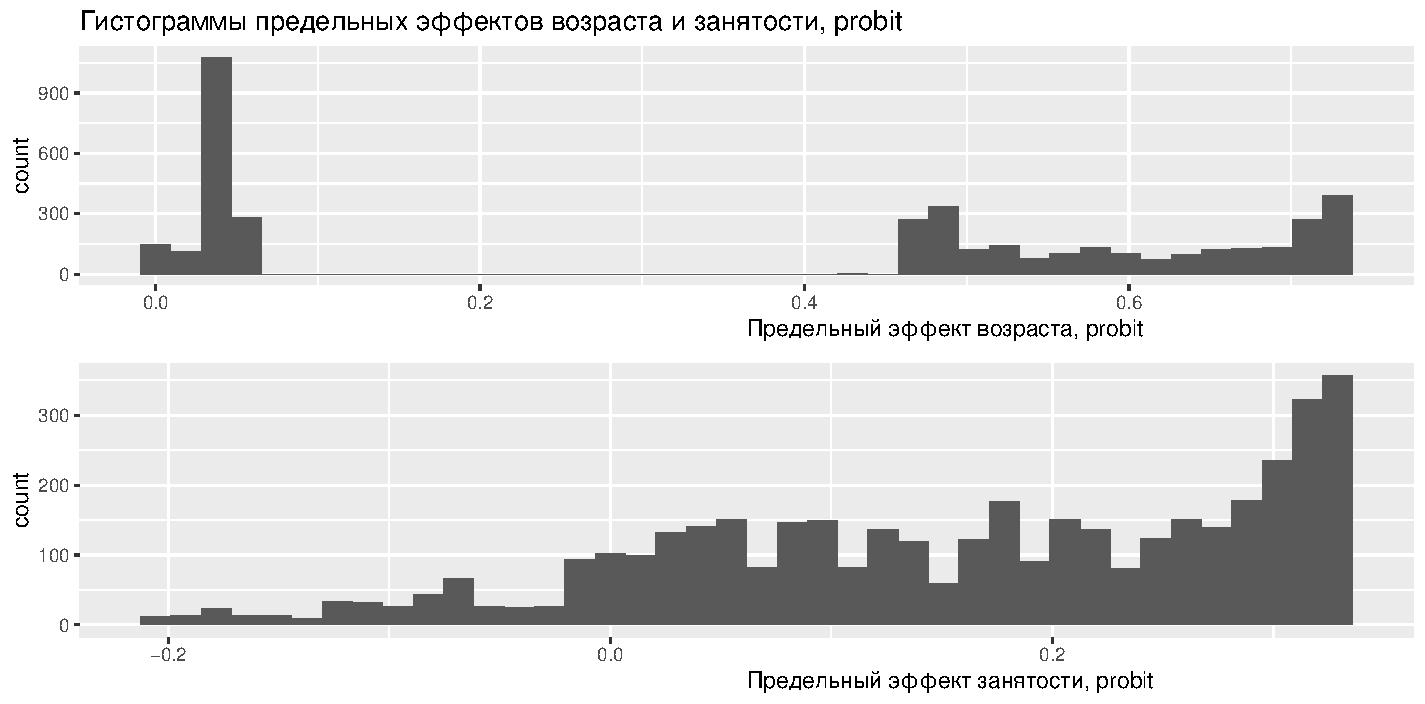
\includegraphics[width=\linewidth]{me_probit}
	\caption{ \label{his2}}
\end{figure}


\subsection{}
 Посчитайте стандартные ошибки оценок предельных эффектов независимых
переменных, входящих в регрессионное уравнений нелинейно, для индивида с вашими
характеристиками, предварительно пояснив методологию расчета.

Подсчитаем дисперсию предельного эффекта.

\[ \Var((\b_1 + 2\b_2 age_i + \b_4 work_i)f(latent\_value_i)) = (\Var(\b_1) + 2 age^2 \Var(\b_2) + work_i^2 \Var(\b_4) +\]

\[  4 age_i \cov(\b_1, \b_2) + 2 work_i \cov(\b_1, \b_4) + 4 age_i work_i \cov(\b_2, \b_4)) * f(latent\_value_i)^2 \]

Подставляя на место истинных дисперсий оценки, получим оценку дисперсии предельных эффектов. Для индивида с моими характеристиками (см. Таблицу 10), корень из этой дисперсии равен 0.0004876624.

\subsection{}

\Sun  Посчитайте значения оценок среднего предельного эффекта, предельного
эффекта для среднего индивида, предельного эффекта для медианного индивида и
предельного эффекта для индивида с вашими характеристиками для каждой из
независимых переменных, представив результат в форме таблицы

Средний предельный эффект, предельные эффекты для среднего и медианного индивидов, а такэе предельные эффекты для меня представлены в Таблице 12
\begin{table}[ht]
	\centering
	\begin{tabular}{|lrr|}
		\hline
		& Age & Work \\ 
		\hline
		Mean ME & 0.3805 & 0.1615 \\ 
		ME of mean person & 0.4517 & 0.2084 \\ 
		ME of median person & 0.3864 & 0.1975 \\ 
		ME of Me & 0.0079 & 0.2005 \\ 
		\hline
	\end{tabular}
\caption{Предельные эффекты: средний, для среднего и медианного индивидов и меня}
\end{table}

\subsection{}



\subsection{}
\Sun  Посчитайте долю верных предсказаний и сопоставьте её с результатом
наивного прогноза. Сделайте вывод о предсказательной силе полученной модели

Из Таблицы 13 очевидно, что прогнозная сила probit-модели заметно выше наивной, но ниже линейной.

\begin{table}[ht]
	\centering
	\begin{tabular}{|rrr|}
		\hline
		& Probit & Naive \\ 
		\hline
		Accuracy & 0.6684 & 0.6118 \\ 
		\hline
	\end{tabular}
	\caption{Доля верных прогнозов моделей}
\end{table}



\subsection{}
\Sun  Посчитайте значение оценки вероятности брака для индивида с вашими
характеристиками. Если вы оцениваете модель по представителям противоположного
пола, то оцените соответствующую вероятность для индивида с вашими
характеристиками, но противоположного пола.


Ответ. Для индивида с характеристиками, представленными в Таблице 10, прогноз равен 0.0653

\section{}
\subsection{}
\Sun При помощи LM-теста протестируйте гипотезу о соблюдении допущения о
распределении случайных ошибок: при этом необходимо формально записать нулевую и
альтернативную гипотезы, статистику теста и её распределение. Запишите, к каким
негативным последствиям может привести нарушение данного допущения.


Ответ. Без предположения о нормальности модель, оценённаяя методом максимального правдоподобия, даст смещённые и несостоятельные оценки. Это очевидно следует из того, что правдоподобие оцениваемой модели будет отличаться от правдоподобия истинной модели.

Пусть $ x_i $ - вектор характеристик i-го индивида ($ Intercept $ $  Age  $ $ Age^2 $ $ Work  $ $ Workxage $), а $ \b $ - вектор коэффициентов. $ y_i $ - бинарная переменная, семейное положение индивида. 

\[ \mathbb{P}\left\{y_{i}=1\right\}=F\left(x_{i}^{\prime} \beta+\gamma_{1}\left(x_{i} ; \beta\right)^{2}+\gamma_{2}\left(x_{i} ; \beta\right)^{3}\right) \]

$ H_0: \gamma_1 = 0, \gamma_2 = 0 $

$ H_A: \gamma_1 \neq 0$ or/and $ \gamma_2 \neq 0 $

Статистика теста:

\[ nR^2 \sim \chi^2_2 \]

где $ R^2 $ из регрессии вектора единиц на вектора первых производных функции правдоподобия каждого индивида по $ \beta, \gamma_1, \gamma_2 $ (каждый вектор - n-мерный):

\[ \ln L_{i}=\ln F\left(x_{i}^{\prime}, \beta+r_{i}\left(x_{i}^{\prime} \beta\right)^{2}+\gamma_{i}\left(x_{i}^{\prime} \beta\right)^{3}\right)^{y_{i}} \cdot (1-F(\cdots))^{1-y_{i}} \]
\subsection{}

\Sun Предположите, какие переменные могут влиять на дисперсию случайной
ошибки. При помощи LR и LM тестов протестируйте гипотезу о гомоскедастичности
случайных ошибок: при этом необходимо формально записать нулевую и альтернативную
гипотезы, статистику теста и её распределение. Запишите, к каким негативным
последствиям может привести нарушение данного допущения. Объясните преимущество
LM теста над LR тестом в данном случае.


Ответ. Предположим, что гетероскедастичность в модели порождается переменной $ Age $. Например, можно предположить, что в молодом возрасте индивиды более склонны создавать или разрушать семьи, то есть изменять своё семейное положение. Люди старшего возраста интуитивно более инертны в этом плане. Следственно, предполагаем, что дисперсия случайных ошибок будет ниже с ростом возраста. Для визуальной проверки этого предположения построим график квадратов остатков probit-модели, агрегированных (суммированием) по возрастам. Как видно из Рис. 3 , этот ряд убывает с ростом возраста. Игнорирование факта наличия гетероскедастичности может привести к неэффективности оценок коэффициентов.

\begin{figure}[!h]
	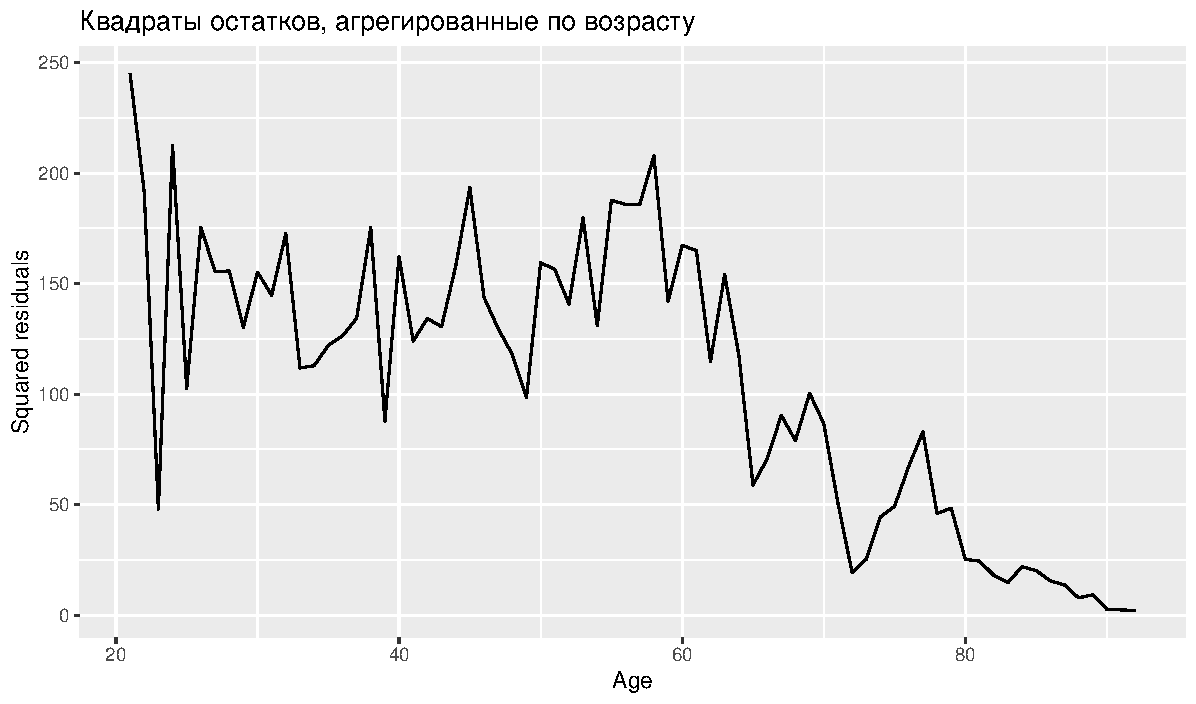
\includegraphics[width=\linewidth]{het_age}
	\caption{ \label{his2}}
\end{figure}



\subsubsection{LR-тест}

Неограниченная модель - Hetprobit

Ограниченная модель - Probit 

$ H_0 $ - гомоскедастичность $\to $ модели эквивалентны

$ H_A $ - отсутствие гомоскедастичности, необходима Hetprobit-модель.

Тестовая статистика: 

\[ LR = 2(lnL_{UR} - lnL_{R}) \sim \chi^2_1\]

Df = 1 так как накладывается всего одно линейное ограничение на Hetprobit-модель, а именно, равенство коэффициента перед Age нулю в уравнении дисперсии.

По результатам теста нулевая гипотеза отвергается, так как p-value = 0
\subsubsection{LM-тест}


Пусть $ x_i $ - вектор характеристик i-го индивида ($ Intercept $ $  Age  $ $ Age^2 $ $ Work  $ $ Workxage $), $ z_i $ - вектор характеристик, подозреваемых в порождении гетероскедастичности, а $ \b $ - вектор коэффициентов. $ y_i $ - бинарная переменная, семейное положение индивида. 

$ \Var(\e_i) = h(x_i^{\prime})k, h(0) = 1^{\prime}, h^{\prime}(0) \neq 0 $


$ H_0: \alpha = 0 $

$ H_A: \alpha \neq 0 $

Статистика теста:

\[ nR^2 \sim \chi^2_1 \]

где $ R^2 $ из регрессии вектора единиц на вектор первых производных правдоподобия по каждому индивиду UR-модели по $ \b, \alpha $. Одна степерь свободы, так как только одна переменная подозревается в порождении гетероскедастичности. 

\subsection{}

\Sun Предпримите действия для борьбы с гетероскедастичностью, оценив
учитывающую её модель. Сравните знаки и значимости коэффициентов с теми, что были
получены при оценивании модели без учета гетерокедастичности.

Ответ. В Таблицах 14 и 15 приведены резултаты оценки Hetprobit- и Probit-моделей. Как можно видеть, стандартные ошибки всех коэффициентов выросли, а значит могли измениться результаты тестирования значимости коэффициентов. Однако, этого не произошло. Все коэффициенты остались значимы на уровне 1\%. Только у переменной  $ workxage $ слегка выросло p-value.  Теперь, после коррекции гетероскедастичности, оценки стали более эффективными. Знаки коэффициентов не изменились.

\begin{table}[ht]
	\centering
	\begin{tabular}{|rrrrr|}
		\hline
		& Estimate & Std. Error & z value & Pr($>$$|$z$|$) \\ 
		\hline
		(Intercept) & -8.0593 & 1.2591 & -6.4008 & 0.0000 \\ 
		age & 0.2825 & 0.0403 & 7.0155 & 0.0000 \\ 
		I(age\verb|^|2) & -0.0020 & 0.0002 & -8.1554 & 0.0000 \\ 
		work & 2.2055 & 0.4106 & 5.3709 & 0.0000 \\ 
		workxage & -0.0262 & 0.0085 & -3.0761 & 0.0021 \\ 
		\hline
	\end{tabular}

\caption{Результат оценивания Hetprobit-модели}

 \vspace{2em}
	\centering
	\begin{tabular}{|rrrrr|}
		\hline
		& Estimate & Std. Error & z value & Pr($>$$|$z$|$) \\ 
		\hline
		(Intercept) & -5.0420 & 0.2778 & -18.15 & 0.0000 \\ 
		age & 0.1783 & 0.0102 & 17.44 & 0.0000 \\ 
		I(age\verb|^|2) & -0.0014 & 0.0001 & -15.04 & 0.0000 \\ 
		work & 1.6845 & 0.1834 & 9.19 & 0.0000 \\ 
		workxage & -0.0249 & 0.0037 & -6.65 & 0.0000 \\ 
		\hline
	\end{tabular}
\caption{Результат оценивания Probit-модели}

 \vspace{2em}
 
	\centering
	\begin{tabular}{|rrrr|}
		\hline
		& Hetprobit & Probit & Naive \\ 
		\hline
		Accuracy & 0.7276 & 0.6684 & 0.6118 \\ 
		\hline
	\end{tabular}
\caption{Доля верных прогнозов моделей}
\end{table}

\subsection{}
\Sun Сравните долю верных прогнозов пробит модели с гетероскедастичной
случайной ошибкой с долей верных прогнозов, полученных при помощи обычной пробит
модели (для тех, кто работает в STATA, это задание со звездочкой *).

Ответ. Сравним качество прогнозов Hetprobit- и Probit-моделей. В Таблице 16 приведены доли верных ответов для обеих моделей. Как можно видеть, качество существенно возросло, но оно всё ещё не переигрывает линейную модель. 

\subsection{}
\subsection{}
\subsection{}
\Sun При помощи LR теста проверьте, можно ли оценивать совместную модель для
людей с различными уровням образования, либо стоит оценить три различные модели для
индивидов с 1) высшим, 2) средним или средним специальным 3) иным уровнем
образования. При помощи LR теста проверьте, можно ли оценивать совместную модель для
людей с различными уровням образования, либо стоит оценить три различные модели для
индивидов с 1) высшим, 2) средним или средним специальным 3) иным уровнем
образования.

Ответ.

Нулевая гипотеза: Обе модели верны

Альтернативная гипотеза: Ограниченная модель неверна, необходимо использоать неограниченную.

Нулевая гипотеза отвергается, p-value теста = 0.00000005072026. Следовательно, следует оценивать отдельные модели для разных уровней образования и нельзя оценивать общую модель.
	

\subsection{}
\Sun Выберите любые две, желательно незначимых на уровне значимости 10\%
переменные, и при помощи LR теста или теста Вальда проверьте, можно ли исключить их
из модели: при этом необходимо формально записать нулевую и альтернативную
гипотезы, статистику теста и её распределение.


Ответ. 
Неограниченная модель:

\[ \P\{ marriage_i  \} = F(\beta_0 + \beta_1 age_i + \beta_2 age_i^2 + \beta_3 work_i + \beta_4 workxage_i + \e_i) \]

Ограниченная модель:

\[ \P\{ marriage_i  \} = F(\beta_0 + \beta_1 age_i + \beta_2 age_i^2 + \e_i) \]

$ H_0: \b_3 = \b_4 = 0 $

$ H_A:  \b_3 \neq 0 $ or/and $ \b_4 \neq 0 $

Статистика теста:

\[ LR = 2(lnL_{UR} - lnL_{R}) \sim \chi^2_2\]

Две степени свободи хи-квадрата, так как два линейно независимых ограничения в нулевой гипотезе.

p-value теста очень близко к 0. Расчёты выдают 0. Следовательно, нельзя исключать указанный набор переменных, и гипотеза о том, что они в совокупности равны нулю отвергается. Необходимо использовать неограниченную модель.


\section{}

\subsection{}
\Sun  Оцените логит модель, предварительно записав максимизируемую функцию
правдоподобия. Результат представьте в форме таблицы (можно, например, использовать
выдачу из stata, R или python)


Пусть $ x_i $ - вектор характеристик i-го индивида ($ Intercept $ $  Age  $ $ Age^2 $ $ Work  $ $ Workxage $), а $ \b $ - вектор коэффициентов. $ y_i $ - бинарная переменная, семейное положение индивида. Функция правдоподобия:

\[
L=\prod_{i}\left[F\left(x_{i}^{\prime} \beta\right)\right]^{y_{i}}\left[1-F\left(x_{t}^{\prime} \beta\right)\right]^{1-y_{i}}
\]

Максимизируемый логарифм функции правдоподобия

\[
l=\ln L=\sum_{i}\left[y_{i} \ln F\left(x_{i}^{\prime} \beta\right)+\left(1-y_{i}\right) \ln \left(1-F\left(x_{i}^{\prime} \beta\right)\right)\right]
\]

\[
F(u)=\frac{e^{u}}{1+e^{u}}
\]

Результаты оценки логит-модели представлены в Таблице 17


\begin{table}[ht]
	\centering
	\begin{tabular}{|rrrrr|}
		\hline
		& Estimate & Std. Error & z value & Pr($>$$|$z$|$) \\ 
		\hline
		(Intercept) & -8.5719 & 0.5109 & -16.78 & 0.0000 \\ 
		age & 0.3016 & 0.0183 & 16.50 & 0.0000 \\ 
		I(age\verb|^|2) & -0.0023 & 0.0002 & -14.55 & 0.0000 \\ 
		work & 2.9526 & 0.3333 & 8.86 & 0.0000 \\ 
		workxage & -0.0441 & 0.0068 & -6.53 & 0.0000 \\ 
		\hline
	\end{tabular}
\caption{Результаты оценки logit-модели}
\end{table}

\subsection{}
\Sun  Проинтерпретируйте значения оценок изменений в отношениях шанса по
каждой независимой переменной.

Так как для всех индивидов это изменение различно, посчитаем это изменение на моих характеристиках. В результате вычислений при $ \delta = 1$ получим результат, представленный в Таблице 18 
\begin{table}[ht]
	\centering
	\begin{tabular}{|rrr|}
		\hline
		& Age & Work \\ 
		\hline
		Delta ratio & 0.0086 & 0.2526 \\ 
		\hline
	\end{tabular}
\caption{Изменение отношения шансов}
\end{table}

Следовательно, при увеличении моего возраста на год, отношение вероятностей изменится в положительную сторону (либо вероятность брака повысится, либо вероятность отсутствия брака понизится, либо и то, и другое одновременно) на 0.8\%. Аналогично, если я найду работу, то отношение шансов вырастет на 25\%.
\section{}

\subsection{}

\Sun  Оцените систему бинарных уравнений на брак и факт употребления алкоголя,
предварительно определив, какая из этих переменных влияет на другую. Результат
представьте в форме таблицы (можно, например, использовать выдачу из stata, R или
python). Дайте интерпретацию изменениям в оценках коэффициентов по сравнению с
обычной пробит моделью


Ответ. Предположим, что факт употребления алкоголя влияет на вероятность вступления в брак. В данном случае можно предположить различную направленность эффектов, так как неизвестна частота употребления алкоголя. Например, можно предположить, что женщин может отпугивать мужчина, который часто употребляет алкоголь. С другой стороны, люди, которые употребляют алкоголь просто от случая к случаю в компании друзей могут просто считать это видом социальной активности, тем самым завязывая новые знакомства и вступая впоследствии в отношения.

Оценим следующую систему уравнений (запишем, для простоты, в латентных переменных)

\[\begin{cases} 
 marriage^*_i = \beta_0 + \beta_1 age_i + \beta_2 age_i^2 + \beta_3 work_i + \beta_4 workxage_i + \gamma alc_i + \e_{1i} \\
 alc^*_i = \alpha_0 + \alpha_1 age_i + \alpha_2 age_i^2 + \alpha_3 work_i + \alpha_4 workxage_i + \e_{2i}
\end{cases}\]

Результаты оценки системы уравнений можно найти в Таблице 19 и Таблице 20.

\begin{table}[ht]
	\centering
	\begin{tabular}{|rrrrr|}
		\hline
		& Estimate & Std. Error & z value & Pr($>$$|$z$|$) \\ 
		\hline
		(Intercept) & -3.53 & 0.45 & -7.90 & 0.00 \\ 
		age & 0.16 & 0.01 & 12.44 & 0.00 \\ 
		I(age\verb|^|2) & -0.00 & 0.00 & -12.77 & 0.00 \\ 
		work & 1.65 & 0.18 & 9.16 & 0.00 \\ 
		workxage & -0.02 & 0.00 & -6.72 & 0.00 \\ 
		alc & -1.35 & 0.11 & -12.59 & 0.00 \\ 
		\hline
	\end{tabular}
\caption{Оценки коэффициентов первого уравнения системы}
\vspace{2em}
	\centering
	\begin{tabular}{|rrrrr|}
		\hline
		& Estimate & Std. Error & z value & Pr($>$$|$z$|$) \\ 
		\hline
		(Intercept) & -1.20 & 0.18 & -6.61 & 0.00 \\ 
		age & 0.07 & 0.01 & 8.74 & 0.00 \\ 
		I(age\verb|^|2) & -0.00 & 0.00 & -8.43 & 0.00 \\ 
		work & 0.95 & 0.13 & 7.09 & 0.00 \\ 
		workxage & -0.01 & 0.00 & -4.47 & 0.00 \\ 
		\hline
	\end{tabular}
\caption{Оценки коэффициентов второго уравнения системы}
\end{table}

\subsection{}
\Sun Проинтерпретируйте значение оценки коэффициента корреляции между
случайными ошибками рассматриваемых уравнений.


Ответ. Также был оценён коэффициент корреляции между случайными ошибками (theta):
\[ theta = 0.889, CI_theta = (0.523,0.978) \]

Следует заметить также, что коэффициент $ \gamma $ перед переменной $ alc $  в первом уравнении значим. Исходя из этого, а также значимости коэффициента $ \theta $ можно сделать следующие выводы:

\begin{enumerate}[\Sun]
	\item Наличенствует причинно-следственная связь между употреблением алкоголя и вероятностью вступления в брак.
	
	\item Так как коэффициент корреляции случайных ошибок значим, в первом уравнении будет присутствовать эндогенность. Случайные ошибки, включённые в уравнение латентной переменной $ alc $, будут коррелировать с собственными случайными ошибками первого уравнения, что будет порождать эндогенность.
	
	
\end{enumerate}


\section{}
\subsection{}
\Sun  Постройте Рок-Кривые для пробит и логит моделей, а также сравните их
предсказательную силу. Какую из этих моделей лучше использовать для получения
уровня специфичности, равного 0.8? Запишите любой уровень специфичности, при
котором лучше использовать пробит модель, чем логит модель, или поясните, почему
такого уровня специфичности не существует, по крайней мере если в качестве критерия
использовать точность предсказания внутри выборки, на которой осуществлялось
оценивание моделей.

Ответ. ROC-кривые представлены на Рис.4.

ROC-AUC hetprobit = 0.7402

ROC-AUC hetlogit = 0.6177

Accuracy hetprobit = Accuracy hetlogit = 0.727

Так как доли правильных ответов равны, сравним их по ROC-AUC. У hetprobit площадь под ROC-кривой больше, следственно, она предпочтительнее. Даже визуально это видно. hetlogit-модель более прижата к оси y = x. Значит, она склоняется в сторону наивной модели. 

Рассмотрим уровни sensitivity для specificity в районе 0.8. 

Для hetprobit ближайшей точкой будет $ (0.462, 0.798) $. Для hetlogit такой точкой будет $ (0.392, 0.816) $. Очевидно из графика, что hetlogit при приближении к точке specificity = $ 0.8 $ резко не вырастет, так что в данном случае hetprobit-модель позволяет получить больший уровень sensitivity при фиксированной specificity. Следовательно, hetprobit-модель является более предпочтительной. 

Одним из таких уровней специфичности, как раз, является 0.8.





\begin{figure}[!h]
	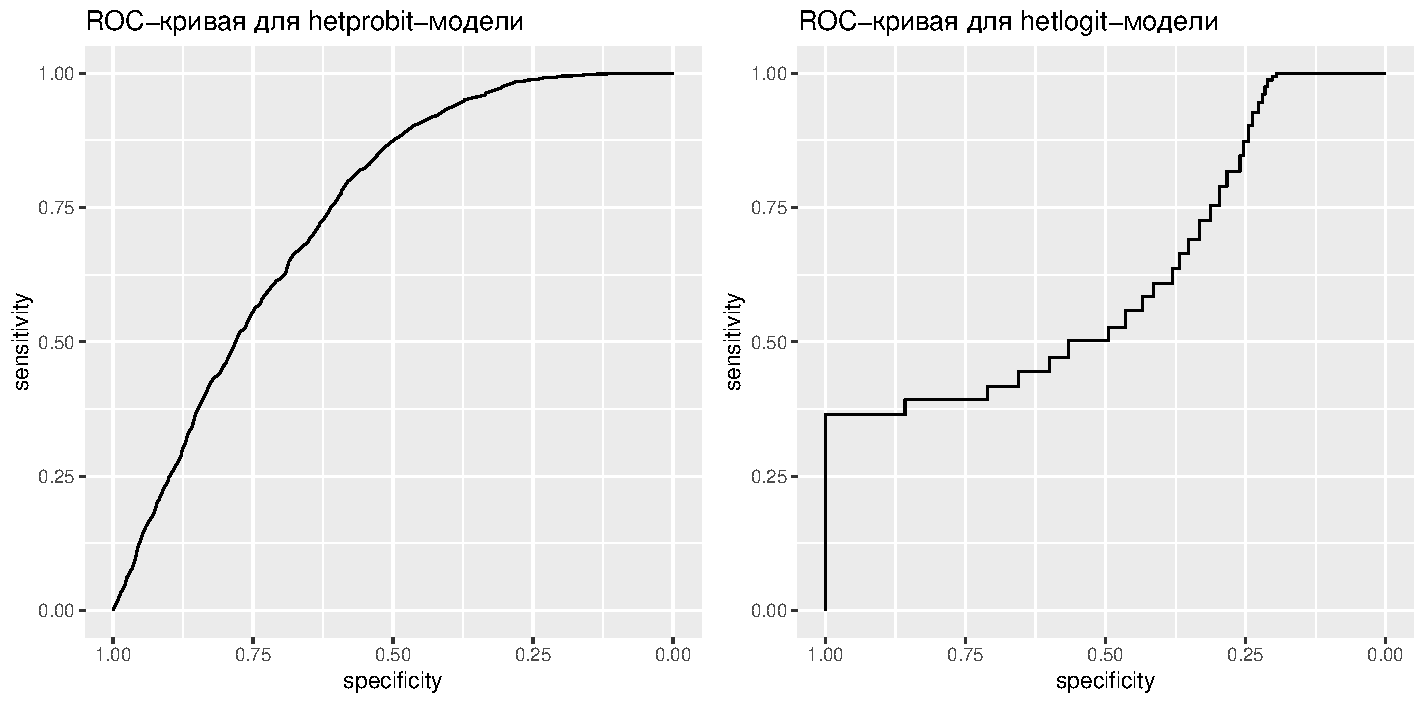
\includegraphics[width=\linewidth]{roc_curves}
	\caption{ ROC-кривые \label{roc}}
\end{figure}

\subsection{}
\Sun Сравните пробит, логит и модель с гетероскедастичной случайной ошибкой по
критериям AIC и BIC, выбрав лучшую из них. Поясните, почему вы не можете сравнить
эти модели по данному критерию с линейно-вероятностной, по крайней мере используя
стандартную выдачу из stata или R

Ответ. Результаты подсчёта информационных критериев представлены в Таблице 21. По обоим информационным критериям побеждает модель с гетероскедастичной случайной ошибкой.  Данные модели нельзя сравнить с линейно-вероятностной моделью, так как для неё неизвестно значение правдоподобия. Она оценивается через МНК, в котором не максимизируется правдоподобие. Следовательно, нельзя вычислить для линейной модели информационные критерии.
\begin{table}[ht]
	\centering
	\begin{tabular}{|rrr|}
		\hline
		Модель & AIC & BIC \\ 
		\hline
		Probit & 4565.54 & 4597.16 \\ 
		Logit & 4566.16 & 4597.78 \\ 
		Hetprobit & 4559.72 & 4597.67 \\ 
		\hline
	\end{tabular}
\caption{Информационные критерии}
\end{table}

\subsection{}

\subsection{}
Разделим выборку на обучающую и тестовую. В последней оставим 500 наблюдений, в первой - все остальные. Обучим на тренировочнонй выборке три модели и посчитаем MSE на тестовой. Получим Результат, представленный в Таблице 22 . Как можно было ожидать, побеждает модель с гетероскедастичной случайной ошибкой. 

\begin{table}[ht]
	\centering
	\begin{tabular}{|rrrrr|}
		\hline
		& Hetprobit & Probit & Logit & Naive \\ 
		\hline
		Accuracy & 0.60 & 0.56 & 0.58 & 0.52 \\ 
		\hline
	\end{tabular}
\caption{Models accuracy}
\end{table}


\end{document}
